\documentclass[14pt, a4paper]{extreport}

\usepackage{susu}

% ====================================================================================================
\begin{document}

\author{Новгородцев~Н.В.}
\group{211}
\task{2}
\maketitle

% ====================================================================================================
\chapter{Задание}

\begin{enumerate}

	\item
	Написать программу для построения пересечения двух прямоугольников. Предполагается, что стороны прямоугольников параллельны координатным осям. Для задания положения и размеров прямоугольников использовать генератор псевдослучайных чисел. Интерфейс программы должен содержать следующие элементы управления:
	\begin{itemize}
		\item создание фигур;
		\item построение решения;
		\item сохранение результата в файл;
		\item выход из программы.
	\end{itemize}

\end{enumerate}

% ====================================================================================================
\chapter{Математическая модель}

Пусть $x_0$, $y_0$, $w$, $h$ -- соответственно координаты левого верхнего угла, ширина и высота прямоугольной области.
При генерации квадратов мы выбираем координаты в диапозоне $x_0$+5 < x < $w$-5 и $y_0$+5 < y < $h$-5.
sq1x1, sq1y1, sq1x2, sq1y2 координаты первого квадрата и sq2x1, sq2y1, sq2x2, sq2y2 координаты второго квадрата.
\par чтобы найти пересечение прямоугольников мы находим его верхний левый $x_1$ $y_1$ и нижний правый угол $x_2$ $y_2$:
$$ x_1 = \left\{ \begin{array}{lr} sq1x1 & sq1x1 > sq2x1\\ sq2x1 & sq1x1 \leq sq2x1 \end{array} \right. $$
$$ x_2 = \left\{ \begin{array}{lr} sq1x2 & sq1x2 \leq sq2x2\\ sq2x2 & sq1x2 > sq2x2 \end{array} \right. $$
$$ y_1 = \left\{ \begin{array}{lr} sq1y1 & sq1y1 > sq2y1\\ sq2y1 & sq1y1 \leq sq2y1 \end{array} \right. $$
$$ y_2 = \left\{ \begin{array}{lr} sq1y2 & sq1y2 \leq sq2y2\\ sq2y2 & sq1y2 > sq2y2 \end{array} \right. $$
Если $x_2 < x_1$ или $y_2 < y_1$ то квадраты не пересекаются\\
Инача закрашиваем квадрат с координами $x_1$ $y_1$ $x_2$ $y_2$


% ====================================================================================================
\chapter{Текст программы}

\noindent Файл main.cpp
\lstinputlisting{source/main.cpp}
\pagebreak
\hrulefill

\noindent Файл task.h
\lstinputlisting{source/task.h}
\hrulefill

\noindent Файл task.cpp
\lstinputlisting{source/task.cpp}
\hrulefill

\noindent Файл control.h
\lstinputlisting{source/control.h}
\hrulefill

\noindent Файл control.cpp
\lstinputlisting{source/control.cpp}

% ====================================================================================================
\chapter{Результат работы}

\begin{figure}[h!]
	\centering
	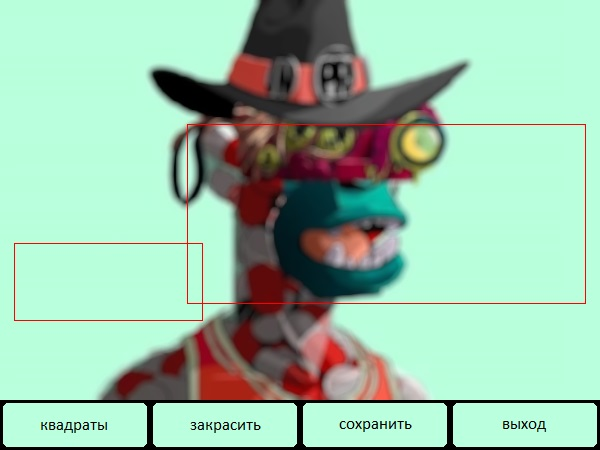
\includegraphics[width = 12cm]{image/output1}
  \caption{Результат выполнения программы (функция creatPoint, кнопка "Установить положение друзей")}
\end{figure}

\begin{figure}[h!]
	\centering
	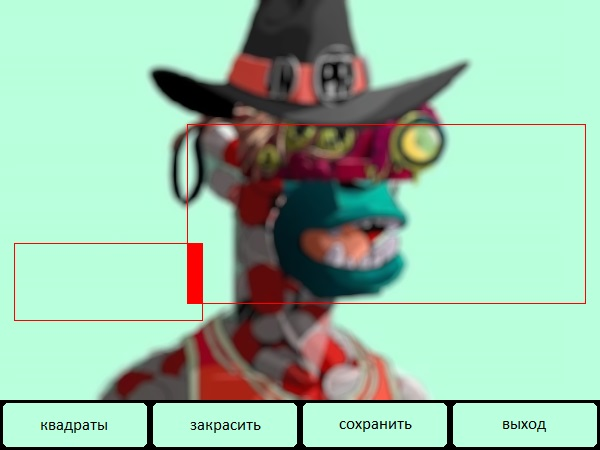
\includegraphics[width = 12cm]{image/output2}
  \caption{Результат выполнения программы (функция treat, кнопка "Найти дальних друзей")}
\end{figure}

% ====================================================================================================
\end{document}